\documentclass{extbook}[14pt]
\usepackage{multicol, enumerate, enumitem, hyperref, color, soul, setspace, parskip, fancyhdr, amssymb, amsthm, amsmath, latexsym, units, mathtools}
\everymath{\displaystyle}
\usepackage[headsep=0.5cm,headheight=0cm, left=1 in,right= 1 in,top= 1 in,bottom= 1 in]{geometry}
\usepackage{dashrule}  % Package to use the command below to create lines between items
\newcommand{\litem}[1]{\item #1

\rule{\textwidth}{0.4pt}}
\pagestyle{fancy}
\lhead{}
\chead{Answer Key for Progress Quiz 1 Version A}
\rhead{}
\lfoot{9226-6023}
\cfoot{}
\rfoot{test}
\begin{document}
\textbf{This key should allow you to understand why you choose the option you did (beyond just getting a question right or wrong). \href{https://xronos.clas.ufl.edu/mac1105spring2020/courseDescriptionAndMisc/Exams/LearningFromResults}{More instructions on how to use this key can be found here}.}

\textbf{If you have a suggestion to make the keys better, \href{https://forms.gle/CZkbZmPbC9XALEE88}{please fill out the short survey here}.}

\textit{Note: This key is auto-generated and may contain issues and/or errors. The keys are reviewed after each exam to ensure grading is done accurately. If there are issues (like duplicate options), they are noted in the offline gradebook. The keys are a work-in-progress to give students as many resources to improve as possible.}

\rule{\textwidth}{0.4pt}

\begin{enumerate}\litem{
Is the following relation a function?


\begin{tabular}{c|c}
x &y\tabularnewline \hline
2 &-20\tabularnewline \hline
3 &-45\tabularnewline \hline
4 &-80\tabularnewline \hline
5 &-80\tabularnewline \hline
4 &20\tabularnewline \hline
3 &45\tabularnewline \hline
2 &80\end{tabular}The solution is No, which is option B.

\begin{enumerate}[label=\Alph*.]
\item Yes

Notice how one $x$-value has two separate outputs? For a relation to be a function, every $x$-value needs exactly one output.
\item No

* Correct! An $x$-value has two separate outputs and thus this relation is not a function.
\end{enumerate}


\textbf{General Comment:} For a relation to be a function, every $x$-value needs exactly one output.
}
\litem{
Is the graph below a linear function?

\begin{center}
    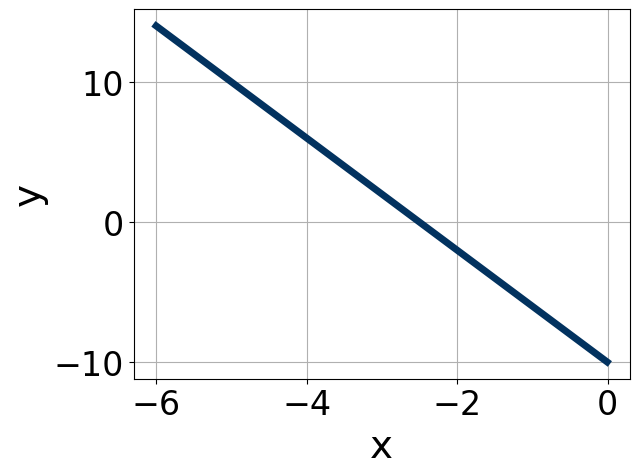
\includegraphics[width=0.5\textwidth]{../Figures/MA_8_F_1_2_graphA.png}
\end{center}


The solution is yes, the graph is linear., which is option A.

\begin{enumerate}[label=\Alph*.]
\item Yes, the graph is linear

* Correct! The graph has a constant rate of change and is thus a linear function.
\item No, the graph is not linear.

A linear function has a constant rate of growth. As $x$ increases/decreases, $y$ increases/decreases at the same rate. The graph in this example does have a constant rate of change.
\end{enumerate}


\textbf{General Comment:} The equation graphed was -4(x + 3)+2. A linear function has a constant rate of growth. This means that as $x$ increases or decreases, $y$ increase or decreases at the same rate. For example, $x^2$ is NOT a linear function. As $x$ increases, the $y$ increases faster and faster. From $x=1$ to $x=2$, the $y$ increases by 3. From $x=2$ to $x=3$, the $y$ increases by 5. From $x=3$ to $x=4$, the $y$ increases by 7. A linear function would have the same change in $y$ for any change in $x$.
}
\litem{
Is the following relation a linear function?


\begin{tabular}{c|c}
x &y\tabularnewline \hline
4 &-64\tabularnewline \hline
5 &-100\tabularnewline \hline
6 &-144\tabularnewline \hline
7 &-196\tabularnewline \hline
8 &196\tabularnewline \hline
7 &64\tabularnewline \hline
6 &100\end{tabular}The solution is No, which is option B.

\begin{enumerate}[label=\Alph*.]
\item Yes

Notice how one $x$-value has two separate outputs? For a relation to be a function, every $x$-value needs exactly one output.
\item No

* Correct! An $x$-value has two separate outputs and thus this relation is not a function, let alone a linear function.
\end{enumerate}


\textbf{General Comment:} For a relation to be a linear function, every $x$-value needs exactly one output AND there needs to be a constant rate of growth (as $x$ increases/decreases, $y$ increases/decreases at the same rate).
}
\litem{
Is the equation below a linear function?
\[ f(x) = -5(x -4)+1 \]The solution is yes, the graph is linear., which is option A.

\begin{enumerate}[label=\Alph*.]
\item Yes, the equation is linear

* Correct! The equation is a degree-1 polynomial and is thus a linear function.
\item No, the equation is not linear.

A linear function is a degree-1 polynomial. Polynomial equations have all variables with positive integer exponents.
\end{enumerate}


\textbf{General Comment:} The equation graphed was -5(x -4)+1. A linear function is a degree-1 polynomial. Polynomial equations have all variables with positive integer exponents, like $f(x) = 3x^2-2x+4$. Square root and cube root functions have rational exponents (1/2 and 1/3).
}
\end{enumerate}

\end{document}